% Abstract for this chapter
%
%**********************************************************************


In this section, we describe the equation of motion of a free-floating base robot.
We derive the equation through the Euler-Lagrange's equation.
Then, we show that the linear/angular conservation laws, which play an important role in robotics,
can be derived from the equation of motion
with assuming invariance of the system Lagrangian under translation and rotation of the entire system.
From linear/angular momentum conservation laws,
we obtain the Reaction Null-Space formulation that 
is useful for reactionless motion control of space robots
and also motion/force control of redundant manipulators.


%%%%%%%%%%%%%%%%%%%%%%%%%%%%%%%%%%%%%%%%%%%%%%%%%%%%%%%%%%%%%%%
\section{Modeling of free-floating base robots}
%%%%%%%%%%%%%%%%%%%%%%%%%%%%%%%%%%%%%%%%%%%%%%%%%%%%%%%%%%%%%%%
%
% ---------------------------------------------------------------------
\begin{figure}[t]
  \centering
  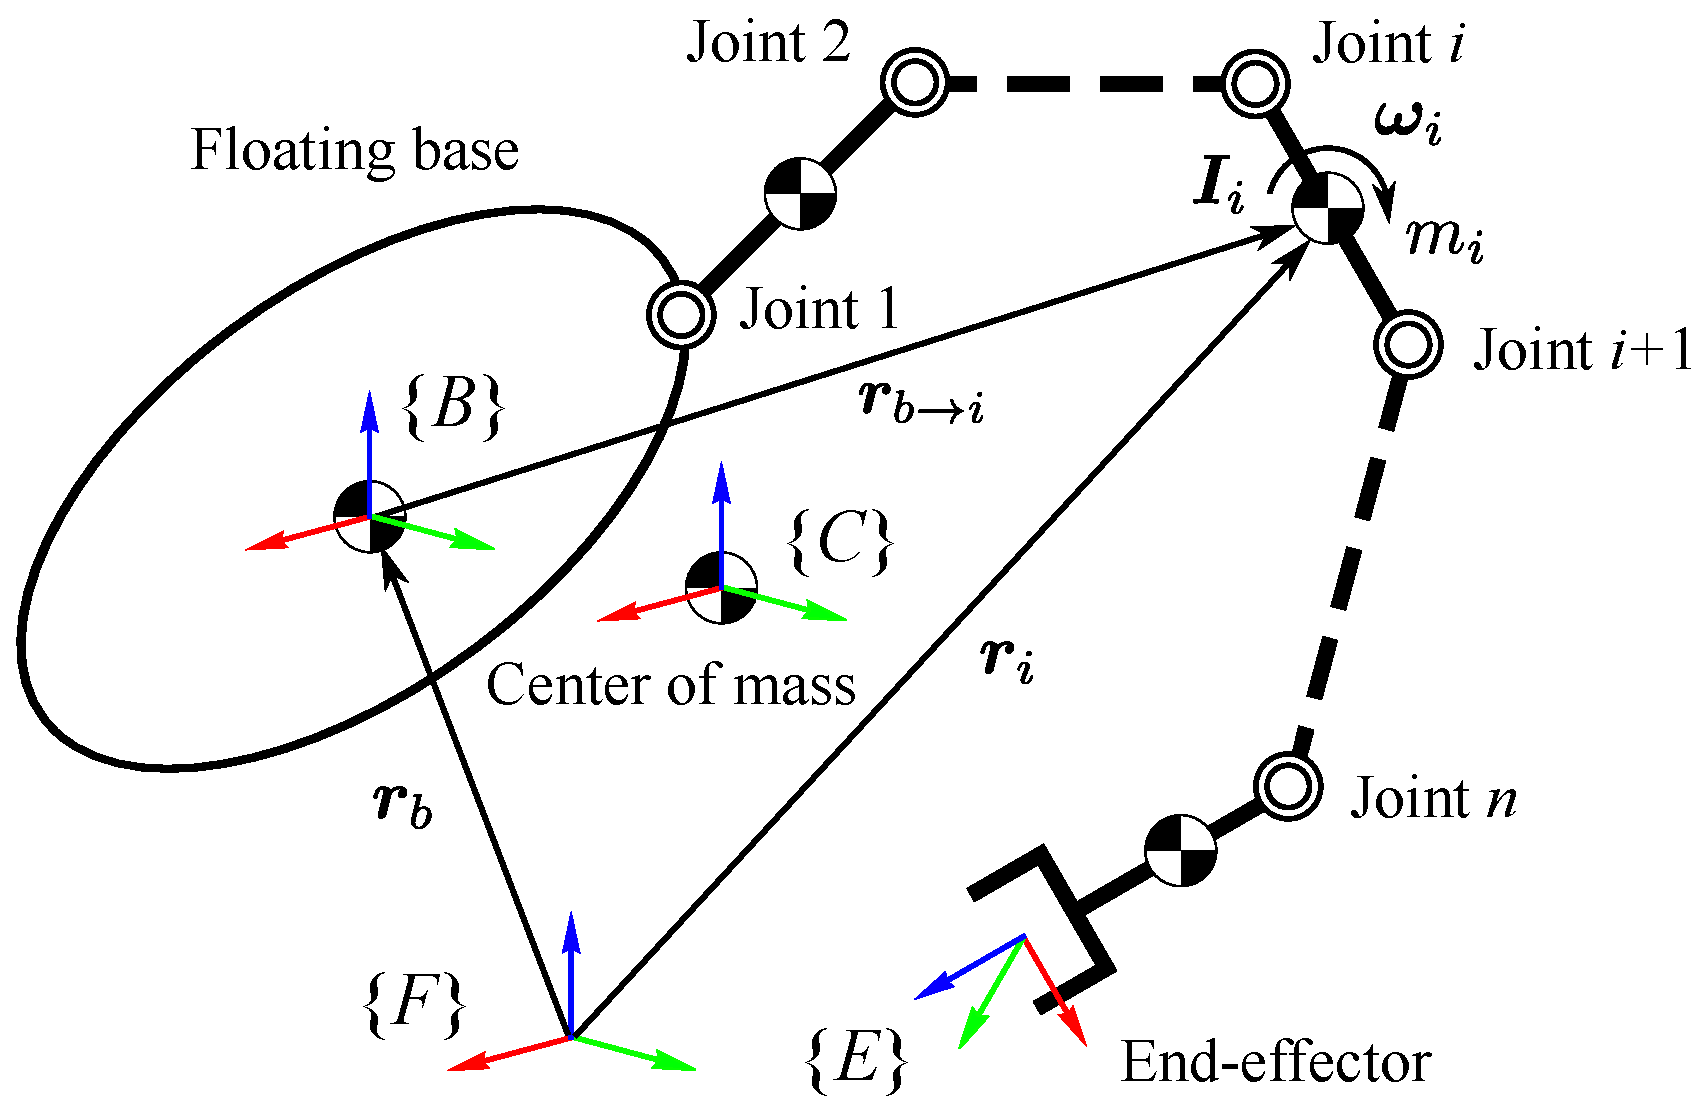
\includegraphics[width=0.7\linewidth]{fig/chapter2/FFSM.eps}
  \caption{General model of free-floating base robot.}
  \label{fig:MODEL_FFSM}
\end{figure}
% ---------------------------------------------------------------------
%
We consider a free-floating base robot 
that consists of a floating base and links, e.g.\ manipulators and reaction wheels,
as shown in \fig{MODEL_FFSM}.
Let us define the inertial coordinate frame $\{F\}$.
% Traditionally, it is considered that the coordinate frame can be moved along the orbit with constant speed.
We use two kind of position vector.
One of them is vector from the inertial frame;
the other is one from the base coordinate frame $\{B\}$.
Note that, except special cases these vectors are described with respect to the inertial frame.


Here, we introduce generalized coordinate to describe the system dynamics.
The coordinate is defined as $\bm{q} = [\mathcal{X}_{b}^{T}~\th^{T}]^{T}\R{n + 6}$,
where $\mathcal{X}_{b} = [\bm{r}_{b}^{T}~\bm{\xi}_{b}^{T}]^{T}\R6$ stands for the base variables:
$\bm{r}_{b}\R3$ and $\bm{\xi}_{b}$ are base position vector and Euler angle describing the base attitude;
especially we make use of Roll-Pitch-Yaw angle.
$\th\R{n}$ is the joint variable vector.
Note that because of the non-integrability of angular velocity,
the base spatial velocity $\mathcal{V}_{b} = [\bm{v}_{b}^{T}~\bm{\omega}_{b}^{T}]^{T}$ cannot be obtained
as the time-differential of $\mathcal{X}_{b}$.
Hence, an appropriate transformation between the time-differential of the Euler angle and the angular velocity is needed:
%
% ---------------------------------------------------------------------
\begin{align}
  \dot{\bm{\xi}}_{b} = \bm{A}^{-1}\bm{\omega}_{b}
\end{align}
% ---------------------------------------------------------------------
%
where $\bm{A}\R{3 \times 3}$ is the transformation matrix.




%%%%%%%%%%%%%%%%%%%%%%%%%
\subsection{Kinematics}
%%%%%%%%%%%%%%%%%%%%%%%%%
Seen from \fig{MODEL_FFSM},
the position vector of each link can be written as follows:
%
% ---------------------------------------------------------------------
\begin{align}
  \bm{r}_{i} = \bm{r}_{b} + \bm{r}_{b \rightarrow i}\label{eq:POS_LINKi}
\end{align}
% ---------------------------------------------------------------------
%
where $\bm{r}_{i}$, $\bm{r}_{b \rightarrow i}$ are the position vectors pointing to the center of mass of each link
from the inertial frame and the base frame, respectively.
Differentiating \eq{POS_LINKi} with respect to time $t$,
we can obtain the differential kinematic equation:
%
% ---------------------------------------------------------------------
\begin{align}
  \bm{v}_{i} = \bm{v}_{b} + \bm{J}_{v_{i}}(\bm{q})\thd + [\bm{\omega}_{b}^{\times}]\bm{r}_{b \rightarrow i}\label{eq:VEL_LINKi}
\end{align}
% ---------------------------------------------------------------------
%
where $\bm{v}_{i}$ stands for linear velocity of link $i$,
$\bm{v}_{b}$, $\bm{\omega}_{b}\R3$ are linear and angular velocities of the base.
$\bm{J}_{v_{i}}(\bm{q})\R{3 \times n}$ is the Jacobian for linear velocity of the link $i$ CoM.
$\dot{(\circ)}$ and $(\circ)^{\times}$ define time differential and skew-symmetric matrix.

In contrast to the linear velocity equation,
the kinematic equation of angular velocity cannot be obtained directly
as the time differential of the position-level equation because of its non-integrability.
The angular velocity of link $i$ is expressed in the following form:
%
% ---------------------------------------------------------------------
\begin{align}
  \bm{\omega}_{i} = \bm{\omega}_{b} + \bm{J}_{\omega_{i}}(\bm{q})\thd\label{eq:ANGVEL_LINKi}
\end{align}
% ---------------------------------------------------------------------
%
where $\bm{\omega}_{i}$ stands for angular velocity of link $i$,
$\bm{J}_{\omega_{i}}(\bm{q})\R{3 \times n}$ is the Jacobian associated with the angular velocity of link $i$.

% For description convenience,
% we introduce spatial velocity $\mathcal{V}_{i} = [\bm{v}_{i}^{T}~\bm{\omega}_{i}^{T}]^{T}$.
% Through the notation,
% the generalized velocity vector can be expressed as $\dot{\bm{q}} = [\mathcal{V}_{b}^{T}~\thd^{T}]^{T}$, hereafter.
% It should be noted that we use Euler angle to represent the orientation of the base
% because of the non-integrability of angular velocity,



%%%%%%%%%%%%%%%%%%%%%%%%%%%%
\subsection{Kinetic energy}
%%%%%%%%%%%%%%%%%%%%%%%%%%%%
The kinetic energy of the free-floating base robots is represented as follows:
%
% ---------------------------------------------------------------------
\begin{align}
  T = \frac{1}{2}\sum_{i = 0}^{n}(m_{i}\bm{v}_{i}^{T}\bm{v}_{i} + \bm{\omega}_{i}^{T}\bm{I}_{i}\bm{\omega}_{i})
  \label{eq:ENERGY_GEN}
\end{align}
% ---------------------------------------------------------------------
%
where $T$ is kinetic energy,
$m_{i}$ and $\bm{I}_{i}\R3$ are the mass and the inertia tensor of each link.
Substituting \eq{VEL_LINKi} and \eq{ANGVEL_LINKi} into the above equation,
we can rewrite the kinetic energy in terms of the base and the joint variables:
%
% ---------------------------------------------------------------------
\begin{align}
  T &= \frac{1}{2}\dot{\bm{q}}^{T}\bm{M}(\bm{q})\dot{\bm{q}}\\
  &= \frac{1}{2}\bmat{\mathcal{V}_{b}^{T} & \thd^{T}}\bmat{\bm{M}_{b}(\bm{q}) & \bm{M}_{bl}(\bm{q}) \\
    \bm{M}_{bl}(\bm{q})^{T} & \bm{M}_{l}(\bm{q})}
  \bmat{\mathcal{V}_{b} \\ \thd}\label{eq:ENERGY}
\end{align}
% ---------------------------------------------------------------------
%
where $\bm{M}(\bm{q})\R{(n+6)\times (n+6)}$ is the inertia matrix of the entire mechanism.
$\bm{M}_{b}(\bm{q})\R{6 \times 6}$,
$\bm{M}_{bl}(\bm{q})\R{6 \times n}$ and $\bm{M}_{l}(\bm{q})\R{n \times n}$ are the submatrices of the inertia matrix;
$\bm{M}_{b}$ is the inertia matrix of the system regarded as a Composite-Rigid-Body (CRB),
$\bm{M}_{bl}$ is a block submatrix of the system inertia matrix.
This matrix represents a dynamic coupling between base motion and link motion.
Hence, it has been referred to as the \textit{coupling inertia} matrix,
and plays an important role under controlling space robots.
Finally, $\bm{M}_{l}$ denotes the manipulator inertia matrix.

%%%%%%%%%%%%%%%%%%%%%%%%%%%%%%%%%%
\subsection{Inertia submatrices}
%%%%%%%%%%%%%%%%%%%%%%%%%%%%%%%%%%
Here, we provide the definitions of the inertia submatrices.
The matrix $\bm{M}_{b}$ is defined in the following form:
%
% ---------------------------------------------------------------------
\begin{align}
  \bm{M}_{b} &= \bmat{\bm{M}_{v} & \bm{M}_{v\omega} \\ \bm{M}_{v\omega}^{T} & \bm{M}_{\omega}}\\
  \bm{M}_{v} &= m_{C}\bm{E}\\
  \bm{M}_{v\omega} &= -\sum_{i=1}^{n}m_{i}[\bm{r}_{b \rightarrow i}^{\times}]\\
  \bm{M}_{\omega} &= \sum_{i=1}^{n}(\bm{I}_{i} + m_{i}[\bm{r}_{b \rightarrow i}^{\times}]^{T}[\bm{r}_{b \rightarrow i}^{\times}]) + \bm{I}_{b}
\end{align}
% ---------------------------------------------------------------------
%
where $m_{C} = \sum_{i=0}^{n}m_{i}$ is the total mass of the system,
$m_{i}$ and $\bm{I}_{i}\R3$ is the mass and the inertia tensor of link $i$.
$\bm{E}\R{3 \times 3}$ is the identity matrix.

The coupling inertia matrix $\bm{M}_{bl}$ is defined as follows:
%
% ---------------------------------------------------------------------
\begin{align}
  \bm{M}_{bl} &= \bmat{\bm{M}_{vl} \\ \bm{M}_{\omega l}}\\
  \bm{M}_{vl} &= \sum_{i = 1}^{n}m_{i}\bm{J}_{v_{i}} = m_{C}\bm{J}_{C}\\
  \bm{M}_{\omega l} &= \sum_{i = 1}^{n}(\bm{I}_{i}\bm{J}_{\omega_{i} } + m_{i}[\bm{r}_{b \rightarrow i}^{\times}]\bm{J}_{v_{i}})
\end{align}
% ---------------------------------------------------------------------
%
where $\bm{J}_{C}\R{3\times n}$ is the Jacobian matrix for the CoM velocity of the system;
hence it is referred to as the CoM Jacobian.

Finally, $\bm{M}_{l}$ is described as follows:
%
% ---------------------------------------------------------------------
\begin{align}
  \bm{M}_{l} = \sum_{i=1}^{n}(m_{i}\bm{J}_{v_{i}}^{T}\bm{J}_{v_{i}} + \bm{J}_{\omega_{i}}^{T}\bm{I}_{i}\bm{J}_{\omega_{i}})
\end{align}
% ---------------------------------------------------------------------
%
Note that this matrix is the same as the manipulator inertia matrix of fixed base robots.


%%%%%%%%%%%%%%%%%%%%%%%%%%%%%%%%%
\subsection{Equation of motion}
%%%%%%%%%%%%%%%%%%%%%%%%%%%%%%%%%
Since we consider free-floating systems,
the gravity potential is approximately zero.
Hence, the system Lagrangian coincides with the kinetic energy:
%
% ---------------------------------------------------------------------
\begin{align}
  L(\bm{q},\dot{\bm{q}}) = T(\bm{q},\dot{\bm{q}})\label{eq:LAGRANGIAN}
\end{align}
% ---------------------------------------------------------------------
%
where $L(\q,\qd)$ is the system Lagrangian.

From the theory of analytical mechanics,
equation of motions of dynamic system can be obtained
from the partial derivation of the system Lagrangian.
Then, equation of motions satisfy the following equation:
%
% ---------------------------------------------------------------------
\begin{align}
  \frac{d}{dt}(\PD{L}{\dot{\bm{q}}}) - \PD{L}{\bm{q}} = \bm{Q}\label{eq:LAGRANGE_EQ}
\end{align}
% ---------------------------------------------------------------------
%
where $\bm{Q}$ is generalized force vector acting on each generalized coordinate.

Substituting \eq{ENERGY} and \eq{LAGRANGIAN} into \eq{LAGRANGE_EQ},
we can obtain the equation of motion of a free-floating base robot in the following form:
%
% ---------------------------------------------------------------------
\begin{align}
  \bm{M}_{b}\dot{\mathcal{V}}_{b} + \bm{M}_{bl}\thdd + \mathcal{C}_{b} &= \bm{0}\label{eq:EOM_BASE}\\
  \bm{M}_{bl}^{T}\dot{\mathcal{V}}_{b} + \bm{M}_{l}\thdd + \bm{c}_{l} &= \bm{\tau}\label{eq:EOM_LINK}
\end{align}
% ---------------------------------------------------------------------
%
where $\bm{\tau}\R{n}$ is joint torque acting on each joint,
$\mathcal{C}_{b}\R{6}$ and $\bm{c}_{l}\R{n}$ are nonlinear
dependent forces of the base and the links.
These nonlinear forces are represented in the following form:
%
% ---------------------------------------------------------------------
\begin{align}
  \bm{c} = \bmat{\mathcal{C}_{b} \\ \bm{c}_{l}} =
  \dot{\bm{M}}\thd - \frac{1}{2}\PD{}{\bm{q}}\Big(\dot{\bm{q}}^{T}\bm{M}\dot{\bm{q}}\Big)
\end{align}
% ---------------------------------------------------------------------
%

Equation \eq{EOM_BASE} represents the dynamics of the composite rigid-body (CRB);
\eq{EOM_LINK} describes the same dynamics with respect to the local coordinate frames.

%%%%%%%%%%%%%%%%%%%%%%%%%%%%%%%%%%%%%%%%%%%
\section{Momentum conservation law}
%%%%%%%%%%%%%%%%%%%%%%%%%%%%%%%%%%%%%%%%%%%
%%%%%%%%%%%%%%%%%%%%%%%%%%%%%%%%%%%%%%%%%%%
\subsection{Linear momentum conservation law}
%%%%%%%%%%%%%%%%%%%%%%%%%%%%%%%%%%%%%%%%%%%

In the field of robotics,
linear and angular momenta and their conservation laws play an important role.
In particular, these provide the reactionless motion constraint for space robots;
in the field of humanoids,
these are used to built balancing controllers and also whole body motion controllers.
Considering the invariance of the system Lagrangian under variations of position and rotation of a dynamic system,
we can obtain the conservation laws in what follows.

First, we derive the linear momentum conservation law of free-floating base robots.
Empirically,
we know that physical laws is not changed with translation of dynamic systems;
the translation indicates that the whole part of the system move in the same direction, simultaneously.

We assume that the system consists of $n+1$ bodies like manipulator mechanisms.
The position vectors pointing to each body are defined as $\bm{r}_{i}$.
Then, under a variation of translation $\delta \bm{r}_{i}$,
the variation of the system Lagrangian can be written as follows:
%
% ---------------------------------------------------------------------
\begin{align}
  \delta L = \sum_{i = 0}^{n}\PD{L}{\bm{r}_{i}}\delta \bm{r}_{i}
\end{align}
% ---------------------------------------------------------------------
%
Because the variation of the Lagrangian muse be zero with an arbitrary value of $\delta \bm{r}_{i}$,
the following condition must satisfy:
%
% ---------------------------------------------------------------------
\begin{align}
  \sum_{i=0}^{n}\PD{L}{\bm{r}_{i}} = \bm{0}
\end{align}
% ---------------------------------------------------------------------
%
According to \eq{LAGRANGE_EQ},
the above condition is equivalent to the following equation:
%
% ---------------------------------------------------------------------
\begin{align}
  \sum_{i=0}^{n}\frac{d}{dt}(\PD{L}{\dot{\bm{r}}_{i}}) = \bm{0}\label{eq:LINEAR_GEN}
\end{align}
% ---------------------------------------------------------------------
%
where $\sum\PD{L}{\dot{\bm{r}}_{i}}$ is an invariable and 
$\bm{p}_{i} = \PD{L}{\dot{\bm{r}}_{i}}$ is defined as \textit{linear momentum}.
Hence, \eq{LINEAR_GEN} represents the linear momentum conservation law.
Using the same expression of \eq{ENERGY_GEN},
the conservation law can be written in the following well-known form:
%
% ---------------------------------------------------------------------
\begin{align}
  \bm{p} = \sum_{i=0}^{n}m_{i}\bm{v}_{i}
\end{align}
% ---------------------------------------------------------------------
%
In the case of free-floating base robots,
a variation of translation can be considered as the base position vector $\delta \bm{r}_{b}$.
Then, the linear momentum conservation law of free-floating base robots can be obtained as:
%
% ---------------------------------------------------------------------
\begin{align}
  \frac{d}{dt}(\PD{L}{\bm{v}_{b}}) = \bm{0}\label{eq:LINE_MOM_LAW}
\end{align}
% ---------------------------------------------------------------------
%
This is equivalent to the following equation:
%
% ---------------------------------------------------------------------
\begin{align}
  \bm{p} = \bm{M}_{v}\bm{v}_{b} + \bm{M}_{v\omega}\bm{\omega}_{b} + \bm{M}_{vl}\thd
\end{align}
% ---------------------------------------------------------------------
%
The above expression of the conservation law has been used in various studies.

%%%%%%%%%%%%%%%%%%%%%%%%%%%%%%%%%%%%%%%%%%%%%%%%%%%%%
\subsection{Angular momentum conservation law}
%%%%%%%%%%%%%%%%%%%%%%%%%%%%%%%%%%%%%%%%%%%%%%%%%%%%%
%
% ---------------------------------------------------------------------
\begin{figure}[t]
  \centering
  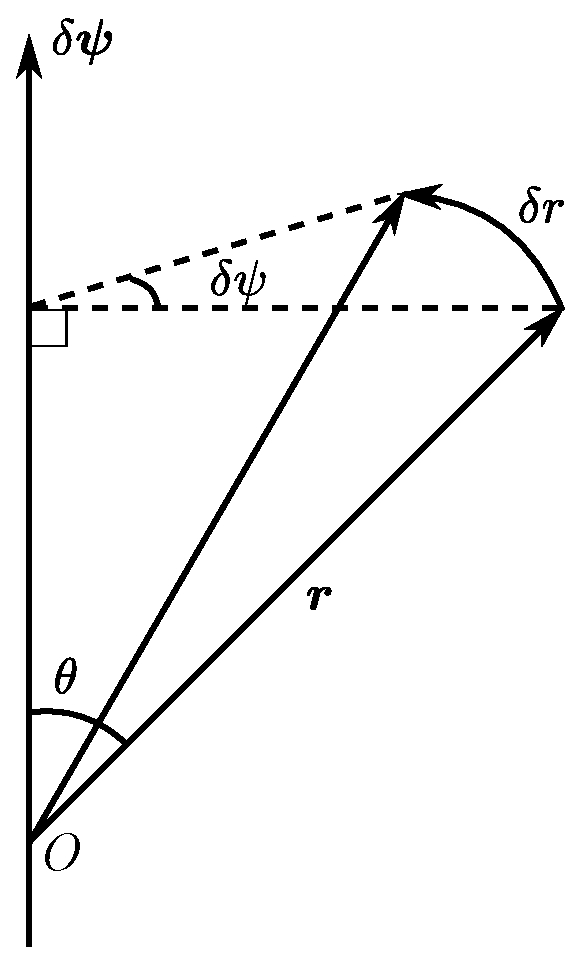
\includegraphics[width=0.3\linewidth]{fig/chapter2/rotation.eps}
  \caption{Relationship between a variation of translation and a rotational variation.}
  \label{fig:ROT}
\end{figure}
% ---------------------------------------------------------------------
%
We derive the angular momentum conservation law of free-floating base robots.
In contrast to linear momentum conservation law,
angular momentum conservation law is obtained from invariance of the system Lagrangian
under an infinitesimal rotation of dynamic systems.

First, we derive, also, the general form of angular momentum conservation law.
We introduce an infinitesimal rotation vector $\delta\bm{\psi}$.
Then, a position vector pointing to an arbitrary particle of a rotating system
varies according to $\delta \bm{\psi}$.
The position variation is written as follows (see \fig{ROT}):
%
% ---------------------------------------------------------------------
\begin{align}
  \|\delta \bm{r}\| = r\sin\alpha\|\delta\bm{\psi}\|
\end{align}
% ---------------------------------------------------------------------
%
Under an arbitrary infinitesimal rotation,
the velocity of each body also varies.
The variation of the velocity is written as:
%
% ---------------------------------------------------------------------
\begin{align}
  \delta \bm{v} = \delta\bm{\psi}\times \bm{v}
\end{align}
% ---------------------------------------------------------------------
%

With the above relation,
the variation of the system Lagrangian under an infinitesimal rotation can be written as:
%
% ---------------------------------------------------------------------
\begin{align}
  \delta L &= \sum_{i=0}^{n}\Big\{\dot{\bm{p}}_{i}(\delta{\bm{\psi}}^{T}\bm{r}_{i}) +
  \bm{p}_{i}(\delta\bm{\psi}^{T}\bm{v}_{i})\Big\}\notag\\
  &= \delta\bm{\psi}\frac{d}{dt}\sum_{i=0}^{n}\bm{r}_{i}\times\bm{p}_{i}\notag\\
  &= 0
\end{align}
% ---------------------------------------------------------------------
%
Because $\delta\bm{\psi}$ can be an arbitrary value,
the following condition muse be satisfied:
%
% ---------------------------------------------------------------------
\begin{align}
  \frac{d}{dt}\sum_{i=0}^{n}\bm{r}_{i}\times\bm{p}_{i} = \bm{0}
\end{align}
% ---------------------------------------------------------------------
%
Hence, we found out that the quantity $\sum\bm{r}_{i}\times\bm{p}_{i}$ conserves;
$\bm{l}_{Fi} = \bm{r}_{i}\times \bm{p}_{i}$ is defined as \textit{angular momentum},
where $(\circ)_{F}$ represent the angular momentum with respect to the inertial frame $\{F\}$.
Using the same expression of \eq{ENERGY_GEN},
we can rewrite the angular momentum conservation law in the following form:
%
% ---------------------------------------------------------------------
\begin{align}
  \bm{l}_{F} = \sum_{i=0}^{n}\Big\{\bm{I}_{i}\bm{\omega}_{i} + m_{i}\bm{r}_{i}\times \bm{v}_{i}\Big\}
\end{align}
% ---------------------------------------------------------------------
%
In the case of free-floating robots,
this equation can be expressed as:
%
% ---------------------------------------------------------------------
\begin{align}
  \bm{l}_{F} = \bm{M}_{v\omega}^{T}\bm{v}_{i} + \bm{M}_{\omega}\bm{\omega}_{b} + \bm{M}_{\omega l}\thd
  + \bm{r}_{b}\times \bm{p}
\end{align}
% ---------------------------------------------------------------------
%

% Summary, momenta conservation laws of free-floating robots can be written as follows:
% %
% % ---------------------------------------------------------------------
% \begin{align}
%   \bmat{\bm{p} \\ \bm{l}_{B}} =
%   \bm{M}_{b}\mathcal{V}_{b} + \bm{M}_{bl}\thd + \bmat{\bm{0} \\ \bm{r}_{b} \times \bm{p}}
%   \label{eq:SPATIAL_MOM}
% \end{align}
% % ---------------------------------------------------------------------
% %



% %%%%%%%%%%%%%%%%%%%%%%%%%%%%%%%%%%%%%%%%%%%%%%%
% \subsection{The momenta conservation law}
% %%%%%%%%%%%%%%%%%%%%%%%%%%%%%%%%%%%%%%%%%%%%%%%


%%%%%%%%%%%%%%%%%%%%%%%%%%%%%%%%%%%%%%%%%%%%
\section{Reaction Null-Space}
%%%%%%%%%%%%%%%%%%%%%%%%%%%%%%%%%%%%%%%%%%%%
Reaction Null-Space was originally proposed for
reactionless motion control of space robots.
With the ETS-VII experiment,
the possibility of reactionless motion control was confirmed.
In what follows, we describe the Reaction Null-Space formulation in terms of both momentum and dynamics.

%%%%%%%%%%%%%%%%%%%%%%%%%%%%%%%%%%%%%%%%%%%%
\subsection{Momentum based derivation}
%%%%%%%%%%%%%%%%%%%%%%%%%%%%%%%%%%%%%%%%%%%%
The spatial momentum conservation law is obtained in the following form:
%
% ---------------------------------------------------------------------
\begin{align}
  \mathcal{L}_{B} = \bm{M}_{b}\mathcal{V}_{b} + \bm{M}_{bl}\thd\label{eq:SPA_MOM}
\end{align}
% ---------------------------------------------------------------------
%
where $\mathcal{L}_{B} = [\bm{p}^{T}~\bm{l}_{B}^{T}]^{T}$ is spatial momentum with respect to the base frame $\{B\}$.
From the above equation,
we can confirm that there are two partial momenta:
$\bm{M}_{b}\mathcal{V}_{b}$ represents the partial momentum related to base motion;
$\bm{M}_{bl}\thd$ is stemming from manipulator motion.
In particular, the later one has been referred to as the \textit{coupling momentum},
and is characterized by the coupling inertia matrix.

Solving \eq{SPA_MOM} for joint velocity,
we can obtain a joint-space decomposition in terms of the dynamic coupling as follows:
%
% ---------------------------------------------------------------------
\begin{align}
  \thd = \bm{M}_{bl}^{+}(\mathcal{L}_{B} - \bm{M}_{b}\mathcal{V}_{b}) + \bm{P}_{RNS}\thd_{a}\label{eq:RNS_VEL}
\end{align}
% ---------------------------------------------------------------------
%
where $(\circ)^{+}$ defines pseudoinverse matrix,
$\bm{P}_{RNS} = \bm{E} - \bm{M}_{bl}^{+}\bm{M}_{bl}\R{n \times n}$ is the projector onto the null-space of
the coupling inertia matrix.
$\thd_{a}\R{n}$ is an arbitrary vector with dimensions of joint velocity.
The first term represents joint velocities inducing a base motion;
on the other hand,
the second term does not impose any motion at the base.
Hence, the motions are referred to as \textit{reactionless motion}.
Since the property of pseudoinverse,
the above two terms are orthogonal with any values of $(\mathcal{L}_{B} - \bm{M}_{b}\mathcal{V}_{b})$ and
$\thd_{a}$.
This joint space decomposition has been referred to as
\textit{Reaction Null-Space} in terms of momentum.


%%%%%%%%%%%%%%%%%%%%%%%%%%%%%%%%%%%%%%%%%%
\subsection{Dynamics based derivation}
%%%%%%%%%%%%%%%%%%%%%%%%%%%%%%%%%%%%%%%%%%
Let us recall the equation of motion \eq{EOM_BASE}, as follows:
%
% ---------------------------------------------------------------------
\begin{align}
  \bm{M}_{b}\dot{\mathcal{V}}_{b} + \bm{M}_{bl}\thdd + \mathcal{C}_{b} &= \bm{0}
\end{align}
% ---------------------------------------------------------------------
%
From the above equation, we can also see that there is
a coupling between the base dynamics and the manipulator one
through the coupling inertia matrix.
Through the same approach under the momentum-based derivation,
the Joint dynamics can be divided into two parts in the following form:
%
% ---------------------------------------------------------------------
\begin{align}
  \thdd = \bm{M}_{bl}^{+}(\bm{M}_{b}\dot{\mathcal{V}}_{b} - \mathcal{C}_{b}) + \bm{P}_{RNS}\thd_{a}\label{eq:RNS_ACC}
\end{align}
% ---------------------------------------------------------------------
%
The first term on the r.h.s.\ represents joint accelerations inducing a base motion,
the second term defines reactionless acceleration, whose meaning is the same as the momentum derivation.
Note that the motions of \eq{RNS_VEL} and \eq{RNS_ACC} are not basically equivalent,
since there is non-integrability between the two formulations;
this non-integrability is due to the pseudoinverse.


%%%%%%%%%%%%%%%%%%%%%
\section{Summary}
%%%%%%%%%%%%%%%%%%%%%
In this section, we described the equation of motion of a free-floating base robots
from the Euler-Lagrange formulation.
We showed the two important conservation laws, which are linear and angular momentum conservation law,
with assuming invariance of the system Lagrangian under variation of position and orientation of dynamic systems.
Then, we derived the Reaction Null-Space formulation with dimensions of both momentum and dynamics.
Joint velocity/acceleration can be divided into two parts through the inertia coupling matrix.
The first part is a motion set inducing a base motion,
the second part does not effect the base motion.
Hence, the second one is referred to as reactionless motion.
Based on this formulation, we will describe reactionless motion of a free-floating space manipulator and
motion/force control for redundant manipulators, in the following sections.



%**********************************************************************
%
%
%%% Local Variables:
%%% mode: latex
%%% TeX-master: "./main"
%%% End: